\graphicspath{{chapters/chapter4/imgs/}}

\chapter{Planowany eksperyment}\label{chapter:ch4}

W tej sekcji przedstawiony zostanie pełny plan eksperymentu, w tym: projekt gry przeglądarkowej
z gatunku \textit{visual novel}, opis implementacji i wykorzystania generatywnych agentów
opartych na dużych modelach językowych oraz sam przebieg badań.

\section{Projekt gry wykorzystanej w eksperymencie}\label{section:ch4_1}

Celem gry ma być oczywiście zbadanie wpływu wykorzystania generatywnych agentów na zaangażowanie
grającego w narrację. W związku z tym rozgrywka powinna kłaść nacisk przede wszystkim na 
przedstawianie treści fabularnych, pozostawiając walory estetyczne czy mechaniki gry na drugim
planie. Dodatkowo, całe doświadczenie powinno mieścić się w przedziale 15-30min i być dostępne
w łatwy sposób (bez instalacji). Z uwagi na te założenia zdecydowano się na utworzenie gry
dwuwymiarowej z gatunku \textit{visual novel} (Patrz sekcja poniżej).

\subsubsection*{Gatunek \textit{visual novel}}\label{subsubsection:ch4_1_1}

Forma \textit{visual novel} (z ang. \textit{powieść wizualna}) jest najczęściej uznawana jako
gatunek gier komputerowych, choć niektórzy dostrzegają w niej zupełnie odrębne od gier 
medium\cite{tvtropes_visual_novel}. 

Kluczowymi cechami \textit{visual novel} są prezentacja tekstu za pomocą okienek dialogowych, które gracz 
musi klikać, aby przejść dalej, oraz statyczne grafiki przedstawiające postacie i otoczenie. Choć 
powieści wizualne często zawierają elementy multimedialne, takie jak animacje, muzyka czy dubbing, 
to nie są one ich kluczowymi składnikami\cite{tvtropes_visual_novel}.

\textit{Visual novel} koncentrują się przede wszystkim na prezentacji narracji, z niewielką lub zerową 
ilością rozgrywki. Wiele z nich oferuje nieliniową, rozgałęziającą się fabułę z wieloma 
zakończeniami i systemem wyborów wpływających na dalszy przebieg wydarzeń\cite{tvtropes_visual_novel}. 
Z drugiej strony, istnieją też powieści wizualne
pozbawione jakiejkolwiek rozgrywki i rozgałęzień fabularnych, określane mianem 
\textit{kinetic novel}\cite{tvtropes_kinetic_novel}.

Ogólnie powieści wizualne wyróżniają się dominacją narracji przedstawianej za pomocą tekstu i grafik nad 
rozgrywką. Kryterium odróżniające je od gier przygodowych jest stopień, w jakim faktycznie 
wykorzystują mechaniki gry i gameplay w stosunku do narracji\cite{tvtropes_visual_novel}.

\subsubsection*{Projekt gry}

Gra została opracowana przy wykorzystaniu silnika Ren'Py w wersji 8.2.1, opartego na języku Python. 
Ren'Py to popularne narzędzie służące do tworzenia gier tego rodzaju, oferujące zaawansowane 
możliwości pisania scenariuszy, zarządzania obrazami i dźwiękiem oraz tworzenia systemów wyborów 
i rozgałęzień fabularnych.

Wszystkie niezbędne zasoby graficzne pozyskane zostały ze społeczności twórców niezależnych na 
platformie itch.io. Grafiki postaci i tła zostały wyprodukowane przez twórców 
LinXueLian (\url{https://linxuelian.itch.io/}) oraz Potat0Master (\url{https://potat0master.itch.io/}), 
specjalizujących się w tego typu materiałach na potrzeby \textit{visual novel} i gier przygodowych.

Po zakończeniu prac, gotowy produkt został wyeksportowany do postaci pliku wykonywalnego 
kompatybilnego z przeglądarkami internetowymi. Takie rozwiązanie umożliwia graczom pobieranie i 
uruchamianie tytułu bezpośrednio ze stron www, bez konieczności instalowania dodatkowego 
oprogramowania.

Finalną wersję gry opublikowano na platformie dystrybucji cyfrowej itch.io, która stała się 
głównym kanałem udostępniania produkcji odbiorcom. Itch.io jest popularnym hubem dla niezależnych 
twórców gier, w tym deweloperów \textit{visual novel} wykorzystujących silniki takie jak Ren'Py.

Na rysunku jest menu bla bla bla.

\begin{figure}[h!]
    \centering
    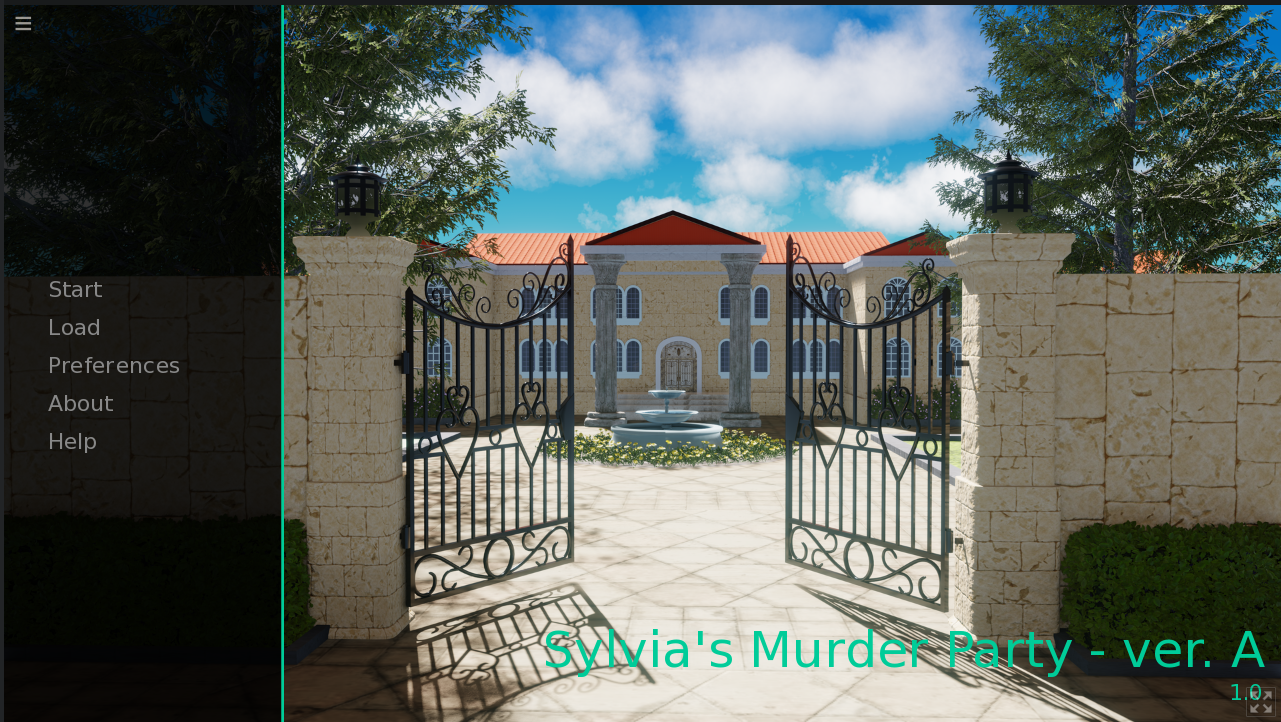
\includegraphics[width=0.9\textwidth]{ch4_1_menu.png}
    \caption{Ekran startowy gry}
    \label{fig:ch4_1_menu}
\end{figure}

\newpage
Na rysunku jest intro i jak to wygląda.

\begin{figure}[h!]
    \centering
    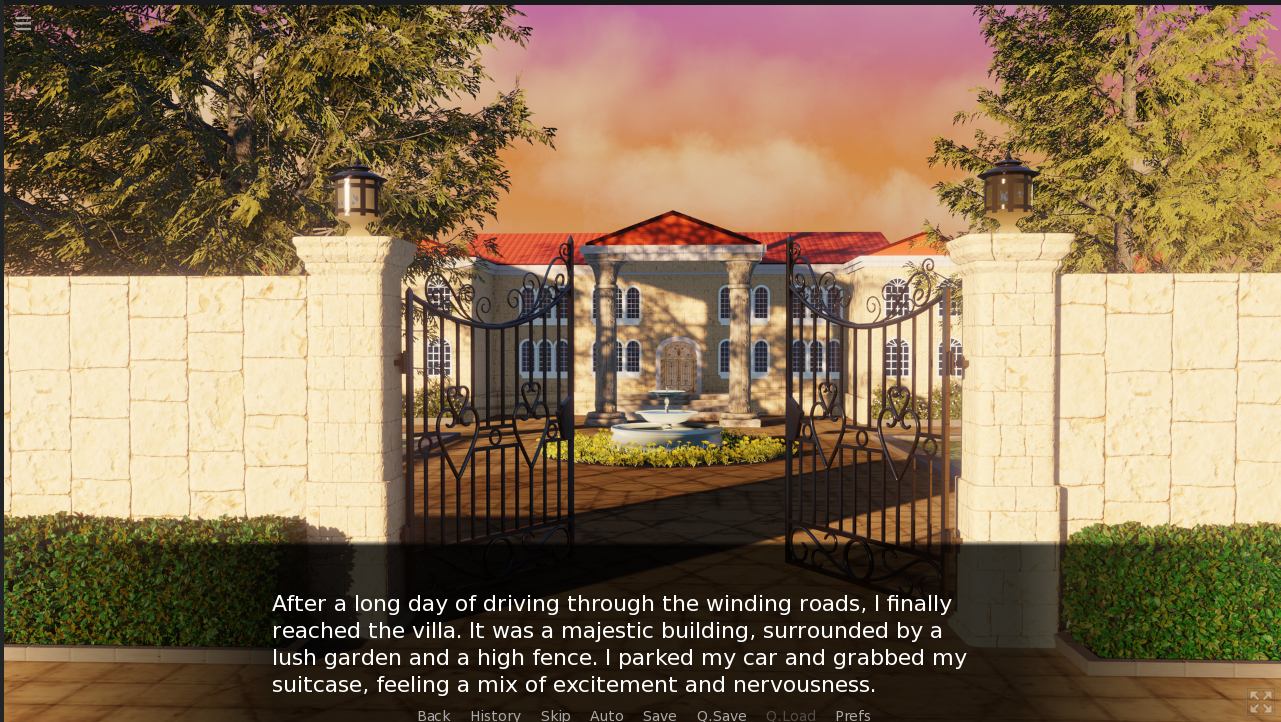
\includegraphics[width=0.9\textwidth]{ch4_1_intro.png}
    \caption{Wprowadzenie fabularne / przykład narracji}
    \label{fig:ch4_1_intro}
\end{figure}

A tutaj dialog przykładowy z postacią NPC.

\begin{figure}[h!]
    \centering
    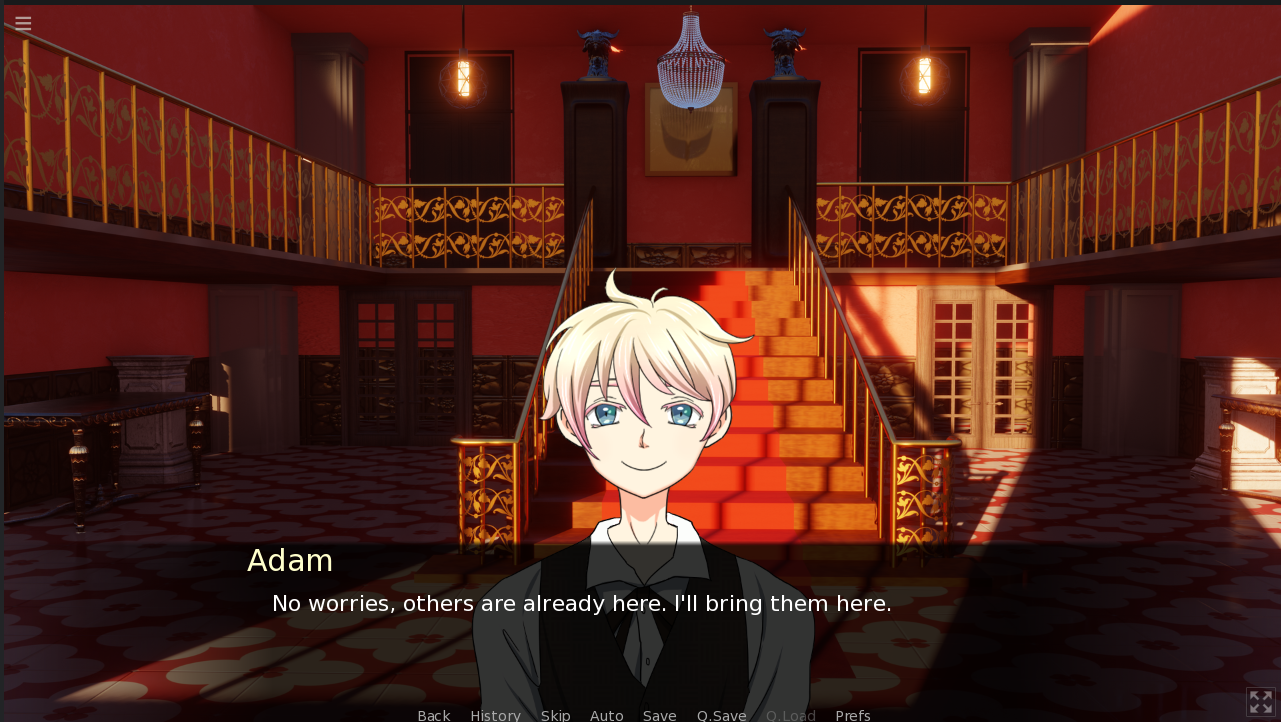
\includegraphics[width=0.9\textwidth]{ch4_1_dialogue.png}
    \caption{Przykładowy dialog z postacią NPC}
    \label{fig:ch4_1_dialogue}
\end{figure}

\subsubsection*{Zarys fabularny}

Gracz zostaje zaproszony na imprezę organizowaną przez Sylvię, bogatą i ekstrawagancką kobietę. Na 
przyjęciu pojawiają się również: Adam - marzyciel pracujący w piekarni ojca, Nathaniel - 
bezwzględny biznesmen, Randy - genialny pianista o ciemnej stronie, Mary - zmagająca się z 
problemami finansowymi pisarka kryminałów oraz Florian - bogaty prawnik zakochany w Sylvii. 
Podczas imprezy Sylvia zostaje zamordowana. Gracz znajduje jej ciało i zostawiony list, który 
sugeruje jej samobójstwo po czym wzywa policję. Do przyjazdu służb potrzeba kilku godzin, więc
główny bohater postanawia samemu rozwiązać tę sprawę. 

Gracz musi rozmawiać z pozostałymi postaciami NPC, zbierając od nich informacje na temat ich 
relacji z Sylvią, motywów i alibi w nocy morderstwa. Adam był skrycie zakochany w Sylvii i 
zazdrosny o jej związek z Florianem. Nathaniel próbował bezskutecznie przejąć piekarnię ojca Adama. 
Randy to utalentowany, ale arogancki pianista z ciemną przeszłością i problemami z prawem, 
skrywający wiele tajemnic. Mary to pisarka kryminałów zmagająca się z problemami finansowymi, 
będąca najlepszą przyjaciółką Sylvii. Florian to bogaty prawnik zakochany w Sylvii, będący rywalem 
Adama w miłości, choć nie zdawał sobie z tego sprawy. Każda postać ma własny charakter i sekrety, 
które mogą okazać się istotne dla śledztwa.

Gra kończy się konfrontacją, podczas której gracz wskazuje sprawcę. 
W zależności od ostatecznego wyboru może być przedstawione "dobre" lub "złe" zakończenie.

\section{Opis generatywnych agentów}\label{section:ch4_2}

faefaef

\subsubsection*{Struktury wykorzystywane przez inworld.ai}

lorfloefleofe

\subsubsection*{Opis wykreowanych postaci}

\textbf{Adam} jest marzycielem z małego miasteczka, który pracuje w piekarni swojego ojca. Marzy o lepszym 
życiu i pragnie wyrwać się z ciasnych ram swojej codzienności. Zna Floriana z liceum i był 
potajemnie zakochany w Sylvii. Czuł zazdrość wobec Floriana z powodu jego relacji z Sylvią. 
Adam nienawidzi Nathaniela, który chce wykupić piekarnię jego ojca. Nie przepada również za 
Randym, którego uważa za aroganta. W nocy, gdy doszło do morderstwa, był przebudzony, obserwując 
Sylvię, i to on znalazł jej ciało.

\textbf{Florian} pochodzi z bogatej rodziny prawniczej. Choć miał wszystko, brakowało mu prawdziwej miłości, 
którą znalazł dopiero w Sylvii. Jest osobą lojalną i gotową do poświęceń dla bliskich. Przyjaźnił 
się z Adamem od czasów liceum, choć nie wiedział o jego uczuciach do Sylvii. Wiedział, że Sylvia 
była najlepszą przyjaciółką Mary. Florian nie lubi Nathaniela za jego metody działania, ale 
podziwia talent Randy'ego, nie wiedząc o jego problemach z prawem. Twierdzi, że spał przez całą 
noc i nie widział Sylvii przed jej śmiercią.

\textbf{Mary} jest pisarką powieści kryminalnych, która zmaga się z finansowymi problemami. Jej najlepszą 
przyjaciółką była Sylvia, która zawsze ją wspierała. Znała Sylvię bardzo dobrze, wiedziała o jej 
depresji i problemach. Była w dobrych stosunkach z Nathaniel'em, który próbował pomóc jej w 
znalezieniu wydawcy. Mary nie ufa Randy'emu i uważa go za podejrzanego. Gdy doszło do morderstwa, 
była w łazience i usłyszała krzyk, ale nie widziała, kto zabił Sylvię.

\textbf{Nathaniel} jest biznesmenem, który dorobił się majątku dzięki swojej determinacji i bezwzględności. 
Pragnie zdobyć szacunek, którego nigdy nie zaznał. Podobał mu się Adam, choć ich relacja była 
napięta z powodu interesów. Nathaniel cenił Randy'ego za jego talent i wierzył, że po odbyciu kary 
więzienia, Randy stał się lepszą osobą. Myślał, że Mary mogłaby zabić z desperacji. Twierdzi, że 
spędził noc w kuchni, widząc Randy'ego palącego papierosy na zewnątrz.

\textbf{Randy} to utalentowany pianista z trudną przeszłością. Choć jest podziwiany za swój talent, jego 
charakter pozostawia wiele do życzenia – jest arogancki i porywczy. Uważał, że Adam jest podejrzany 
z powodu jego zachowania względem Sylvii. Miał mieszane uczucia co do Floriana, którego uważał za 
podejrzanego. Wierzył, że Mary potrzebuje prawdziwej inspiracji do swojej pracy. Twierdził, że 
spędził noc na zewnątrz, paląc papierosy. W rzeczywistości to on zabił Sylvię, choć stara się to 
ukryć.

\subsubsection*{Wykorzystanie agentów w praktyce}

lorfloefleofe

\section{Zaplanowany przebieg eksperymentu}\label{section:ch4_3}

pofkepfokawpefkwpeofk

\subsubsection*{Forma eksperymentu}

lorfloefleofe

\subsubsection*{Gromadzone dane}

lorfloefleofe